% 2007 年天津卷文科第 19 题：四棱锥 P-ABCD，PA ⊥ 底面 ABCD，E 为 PC 中点。
% 来源 PDF：source.pdf，SHA256 f4257944971547472f433b7da4dedb1dad9763fd284397f12daf6cf52c58283a
% 原页：source.pdf 第 1 页（A3 三栏）第 3 栏，书页码 415，图在第 19 题题干下方。
% 重绘依据：按原图的斜二测式透视取点（P 在 A 正上方偏左、A 在左、B 在下方、C 在右下方、
%   D 在最右），可见棱 PA、PB、PC、PD、AB、BC、CD 画实线，被棱锥遮住的底面线 AC、AD 与
%   辅助线 AE 画虚线；E 取 PC 中点（1.80,1.625），BE 按原图为实线，原图不画 DE。
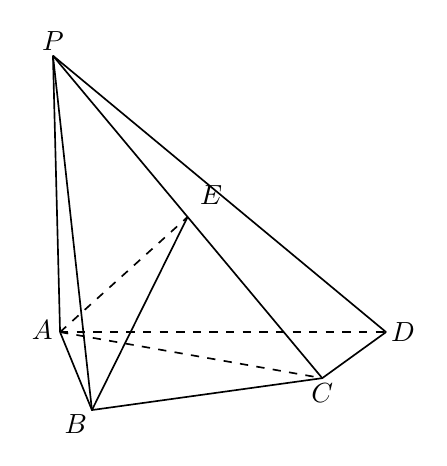
\begin{tikzpicture}[scale=0.9, semithick,
  every node/.style={inner sep=1.5pt}]
  \coordinate (P) at (-0.10,3.90);
  \coordinate (A) at (0,0);
  \coordinate (B) at (0.45,-1.10);
  \coordinate (C) at (3.70,-0.65);
  \coordinate (D) at (4.60,0);
  \coordinate (E) at (1.80,1.625);
  % 底面被遮挡的对角线与辅助线
  \draw[dashed] (A) -- (C);
  \draw[dashed] (A) -- (D);
  \draw[dashed] (A) -- (E);
  % 可见棱与底面可见边
  \draw (A) -- (B) -- (C) -- (D);
  \draw (P) -- (A);
  \draw (P) -- (B);
  \draw (P) -- (C);
  \draw (P) -- (D);
  \draw (B) -- (E);
  \node[anchor=south] at (P) {$P$};
  \node[anchor=east] at ([xshift=-1pt,yshift=1pt]A) {$A$};
  \node[anchor=north east] at (B) {$B$};
  \node[anchor=north] at (C) {$C$};
  \node[anchor=west] at (D) {$D$};
  \node[anchor=south west] at ([xshift=3pt,yshift=3pt]E) {$E$};
\end{tikzpicture}
